We now present the inclusive study performed at NLO QCD, namely $\mathcal{O}(\alpha^6\alpha_s)$.\\
According to the results shown in sec.~\ref{subsec:LOinclusive}, the VBS approximation at LO fails in the region $m_{jj} < 200$ GeV, $|\Delta y_{jj}| < 2$; moreover, we would like to validate this approximation (and its extension to $s$--channels inclusion) at the NLO accuracy. Thus, we impose the same kinematic cuts shown in sec.~\ref{subsec:inputpar} relaxing the VBF cuts and asking for
\begin{equation}
	m_{jj} > 200 \,\textrm{GeV}\,,\qquad |\Delta y_{jj}| > 2\,.
\end{equation}
We compare three different predictions at NLO QCD: {\sc Bonsay} employs the VBS approximation ($|t|^2+|u|^2$), {\sc Vbfnlo} adds the $s--$channel contributions ($|s|^2+|t|^2+|u|^2$) and {\sc Recola} employs full matrix--elements, adding also $t/u$ interferences, factorisable and non--factorisable QCD corrections to the leading electroweak order, as well as the EW correction to the $\mathcal{O}(\alpha^5\alpha_s)$ interference. The total cross--sections within the above mentioned kinematic cuts are shown in table~\ref{tab:crosssecINCLUSIVE}
\begin{table}[h!]
\centering
\begin{tabular}{c|c|c} 
\bf Matrix--element & $\sigma_{\textrm{tot}}\,[\textrm{fb}]$ & $\delta$ \\
\hline
\hline
full &  1.8120 $\pm$ 0.0144 & - \\
\hline
$|t|^2 + |u|^2$ & 1.6292 $\pm$ 0.0001  &  -10 \% \\
\hline
$|s|^2 + |t|^2 + |u|^2$ & 1.7780 $\pm$ 0.0001  & -2 \%
\end{tabular}
\caption{Total cross--sections at NLO QCD $\mathcal{O}(\alpha^6\alpha_s)$, with $m_{jj}>200$ GeV, $|\Delta y_{jj}|>2$.}
\end{table}\label{tab:crosssecINCLUSIVE}


{\bf GP: Comment on the $m_{jj}, \Delta y_{jj}$ distributions, mainly in the region $200 < m_{jj} < 500$ and $2<|\Delta y_{jj}|<2.5$.}
\begin{figure}[hbt]
\centering
{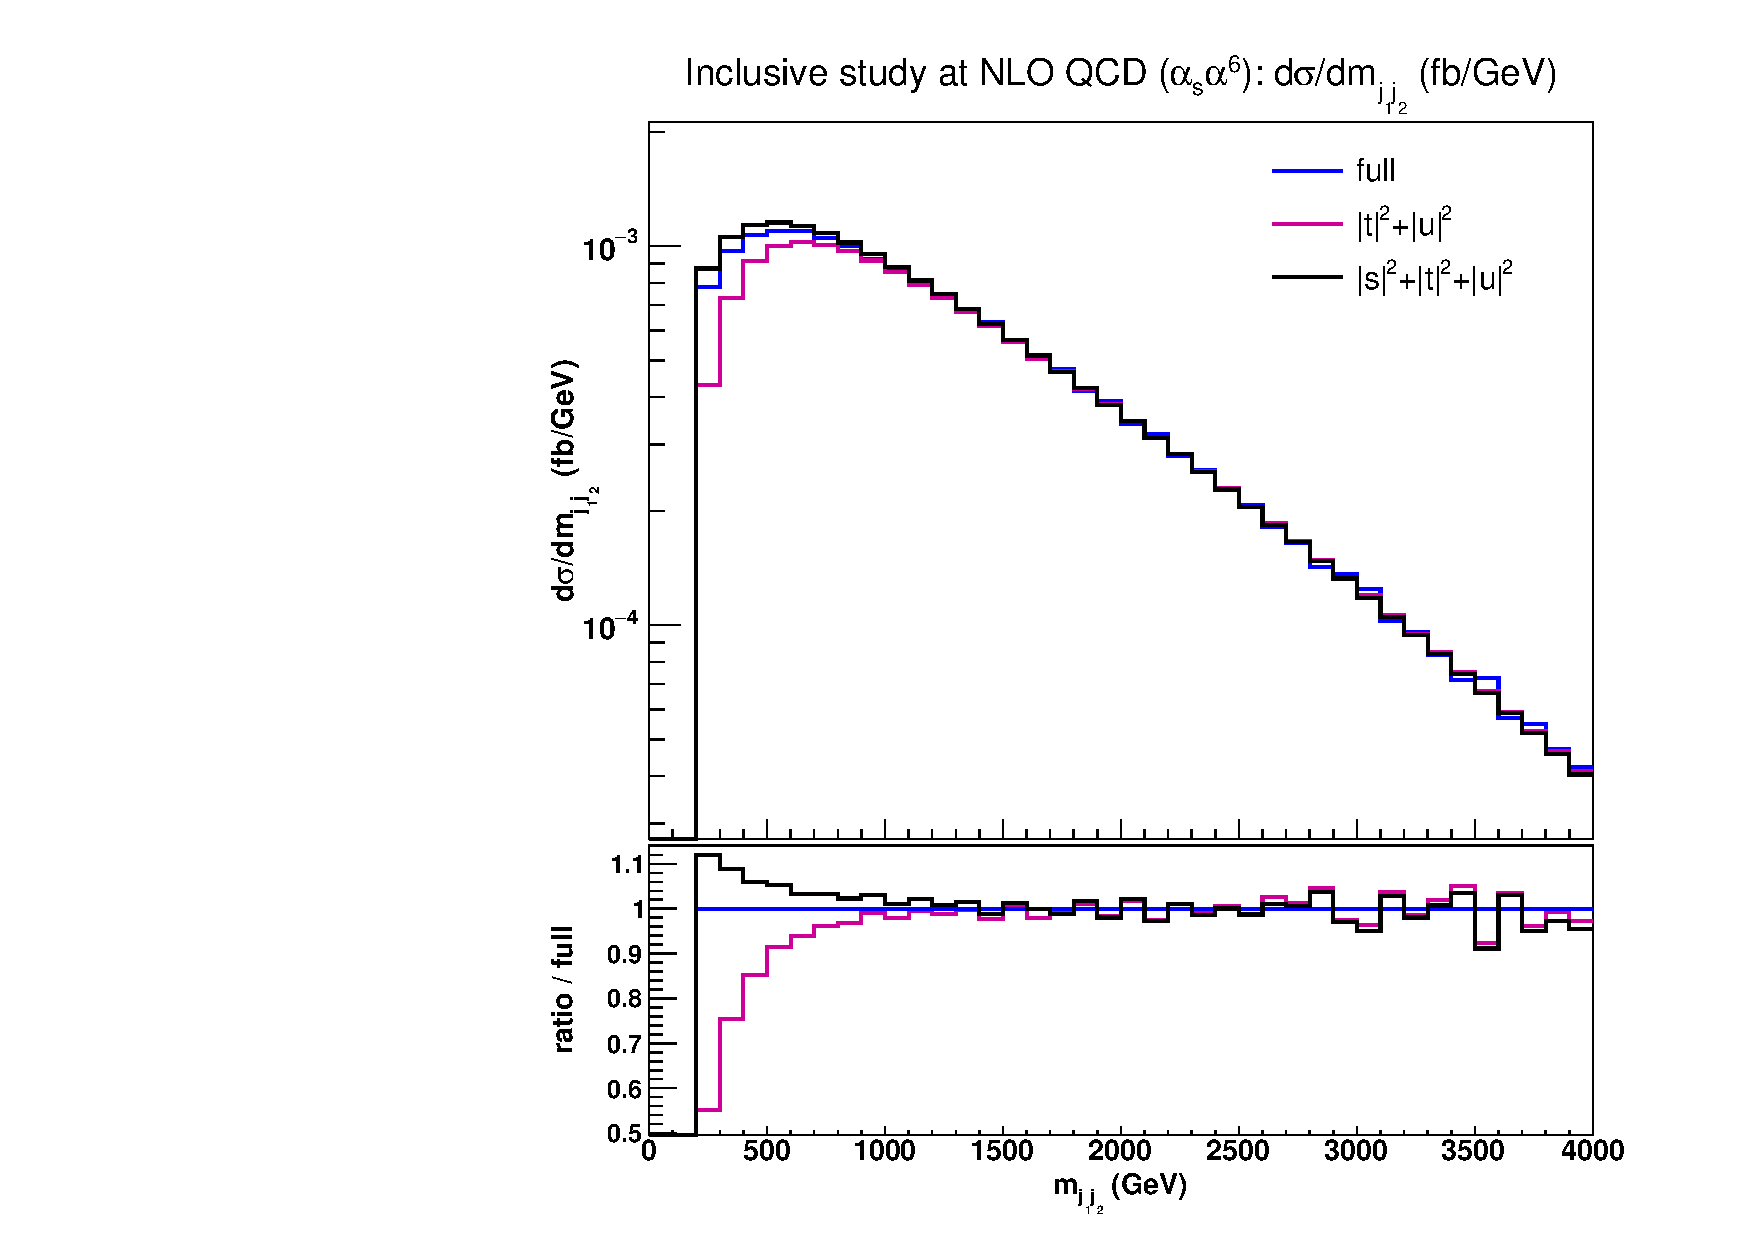
\includegraphics[scale=0.35]{mjj_nlo.pdf}}
{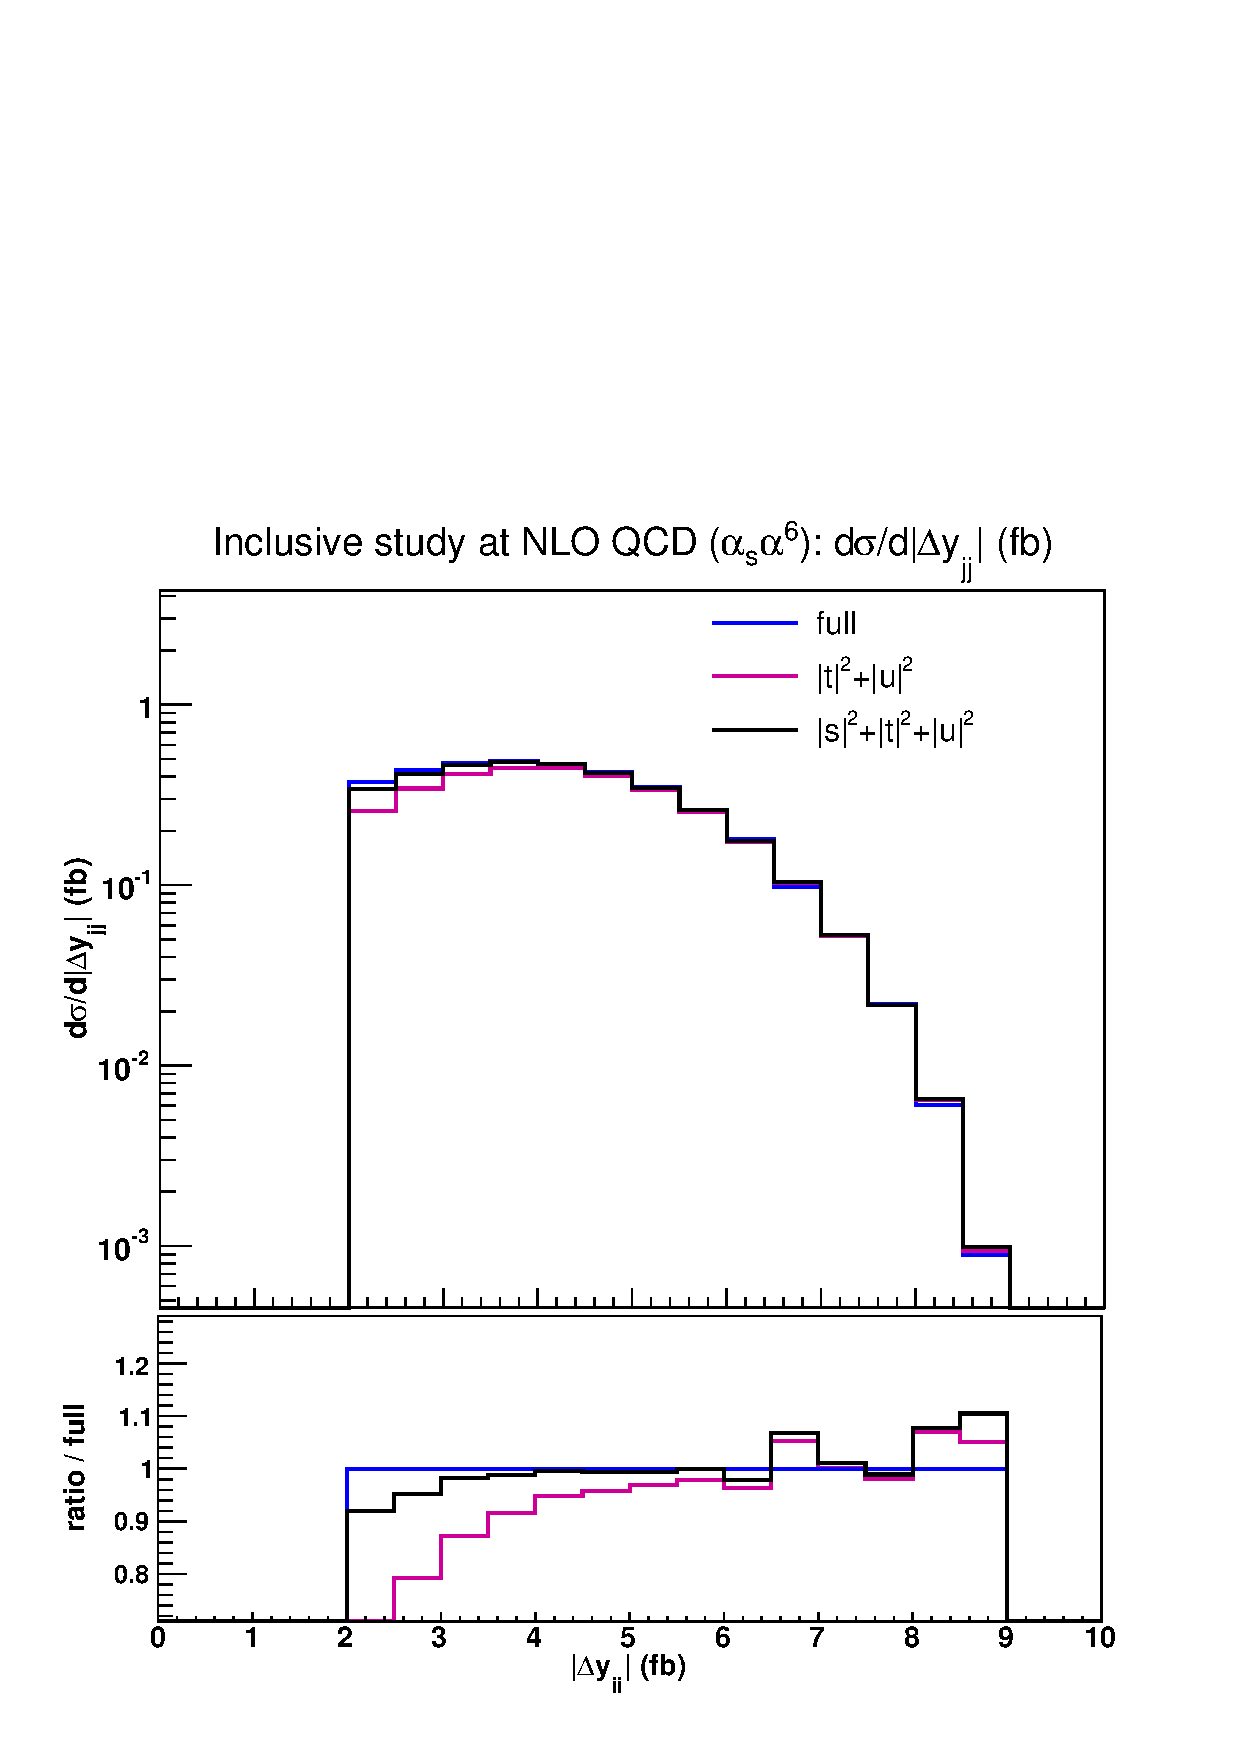
\includegraphics[scale=0.35]{dyjj_nlo.pdf}}
\caption{NLO QCD inclusive study: distributions in $m_{jj}$ (left) and $\Delta y_{jj}$ (right), obtained with full ({\sc Recola}) and approximated ({\sc Vbfnlo, Bonsay}) amplitudes at order $\mathcal{O}(\alpha^6\alpha_s)$.} \label{fig:mjjdyjj_1d_1}
\end{figure}

{\bf GP: Comment on the $m_{jj}, \Delta y_{jj}$ 2D scan: s--channels yes/no, left discrepancies after s--channel inclusion.}
\begin{figure}[h]
\centering
{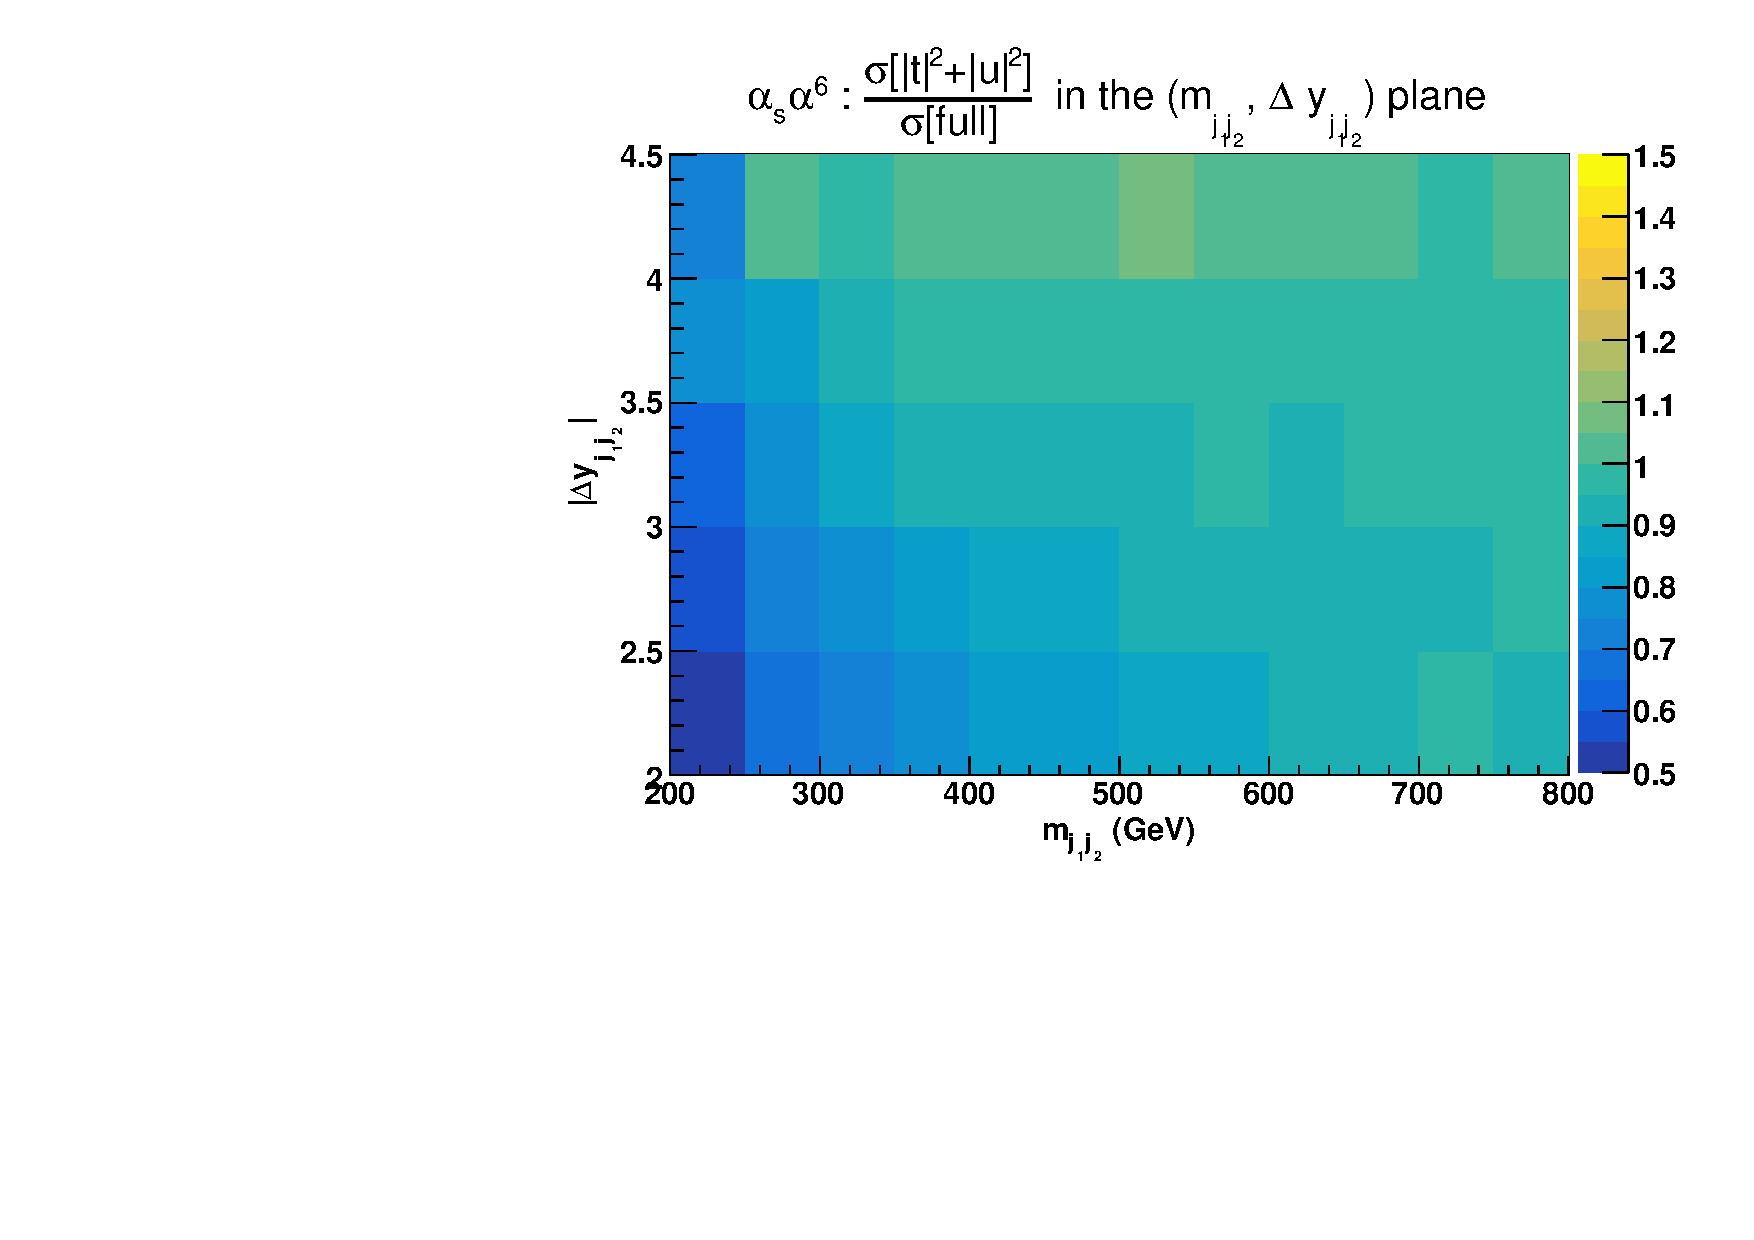
\includegraphics[scale=0.39]{a6as_vbfnloVSrecola_tu.pdf}} 
%\includegraphics[scale=0.395]{figures/scanfigures/.pdf}
\caption{Cross sections (fb) per bin of $(m_{jj},\,\Delta y_{jj})$ at NLO QCD $\mathcal{O}(\alpha^6\alpha_s)$, without any cut on the $jj$ pair kinematics: ratio of approximated squared amplitudes over the full matrix element. The approximated squared amplitudes are computed as $|\mathcal{A}|^2 \sim |t|^2 + |u|^2$. Results of {\sc Vbfnlo} (approximated) and {\sc Recola} (full) calculations.}\label{fig:ratio2d_NLO}
\end{figure}

\begin{figure}[hbt]
\centering
{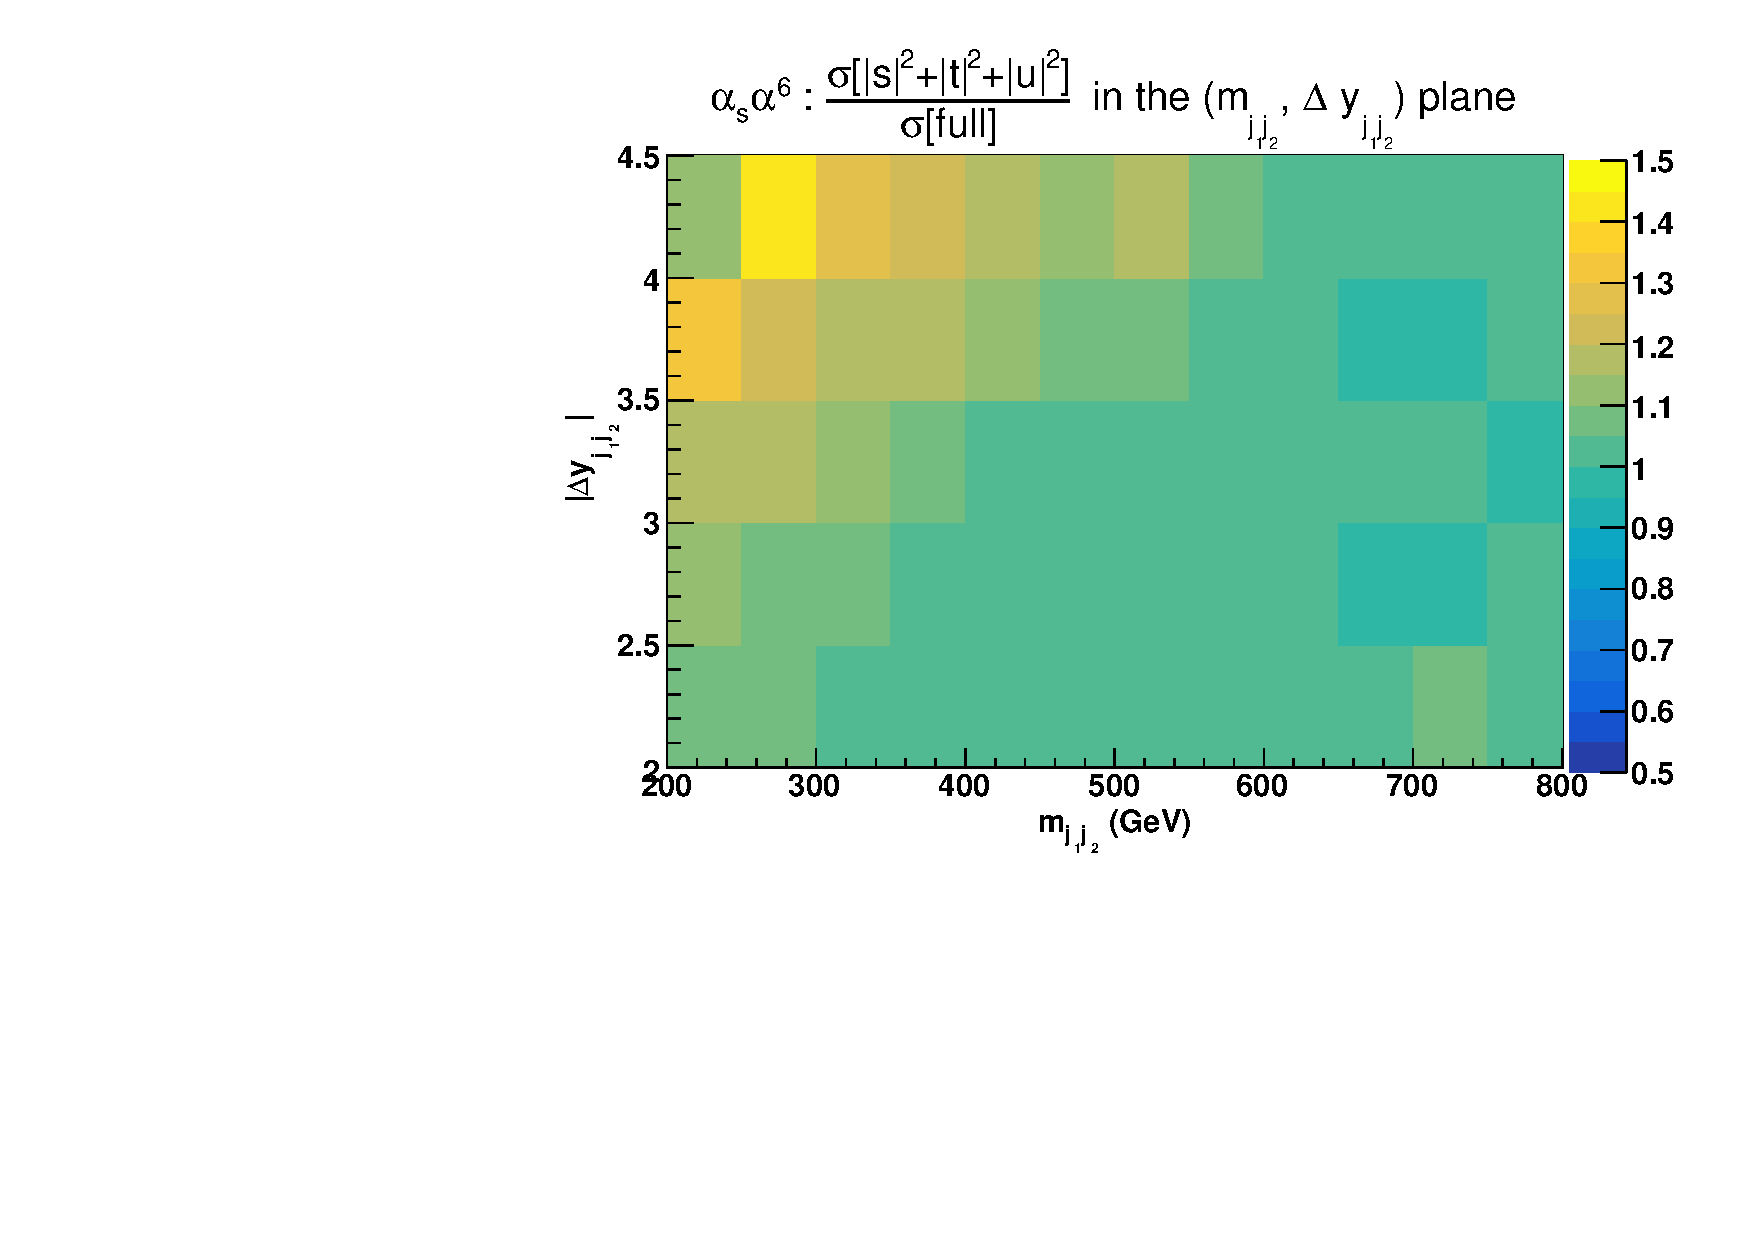
\includegraphics[scale=0.39]{a6as_vbfnloVSrecola_stu.pdf}}
\caption{Cross section (fb) per bin of $(m_{jj},\,\Delta y_{jj})$ at NLO QCD $\mathcal{O}(\alpha^6\alpha_s)$, without any cut on the $jj$ pair kinematics:  ratio of approximated squared amplitudes over the full matrix element. The approximated squared amplitudes are computed as $|\mathcal{A}|^2 \sim |s|^2 + |t|^2 + |u|^2$. Results of {\sc Vbfnlo} (approximated) and {\sc Recola} (full) calculations.}\label{fig:mjjdyjj_2d_NLO}
\end{figure}

{\bf GP: Comment on the other distributions: all the plots ?}
\begin{figure}[hbt]
\centering
{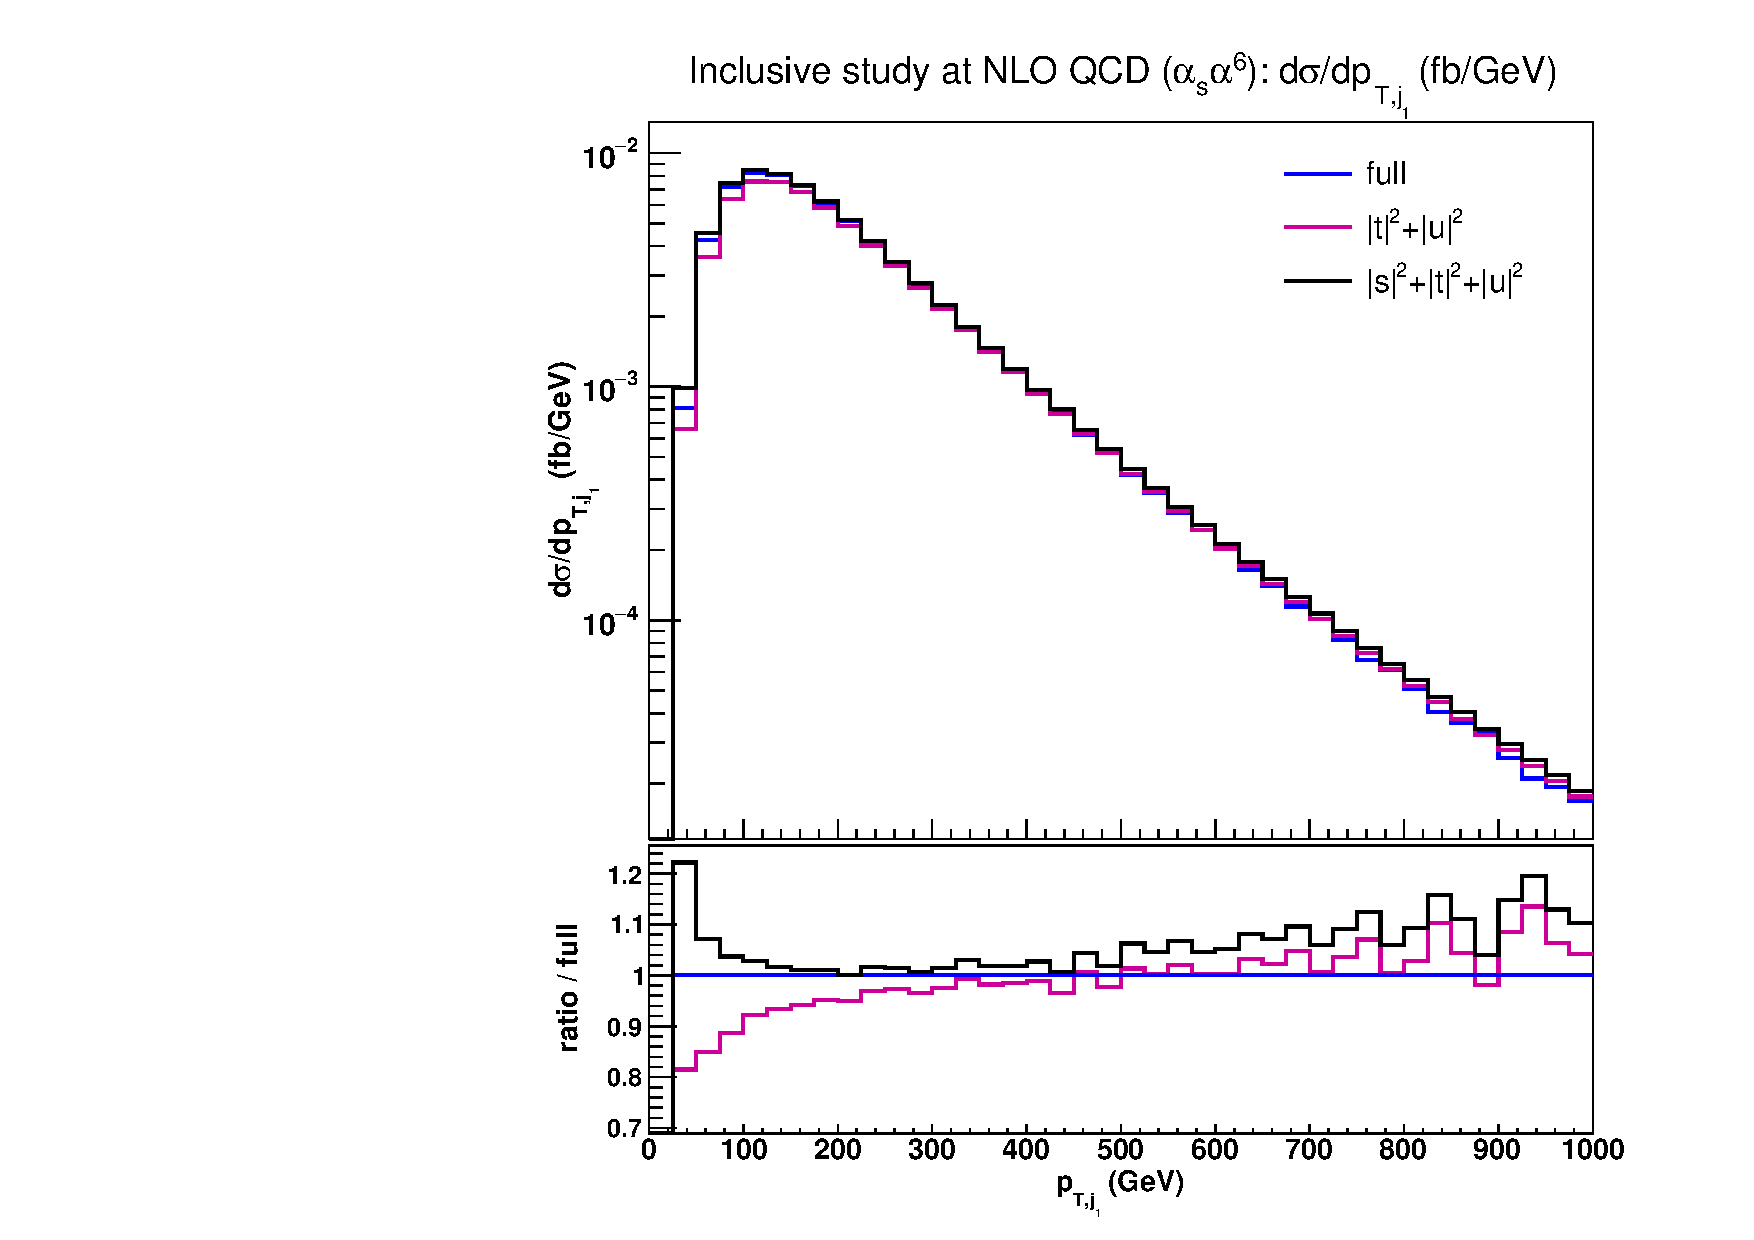
\includegraphics[scale=0.35]{ptj1_nlo.pdf}}
{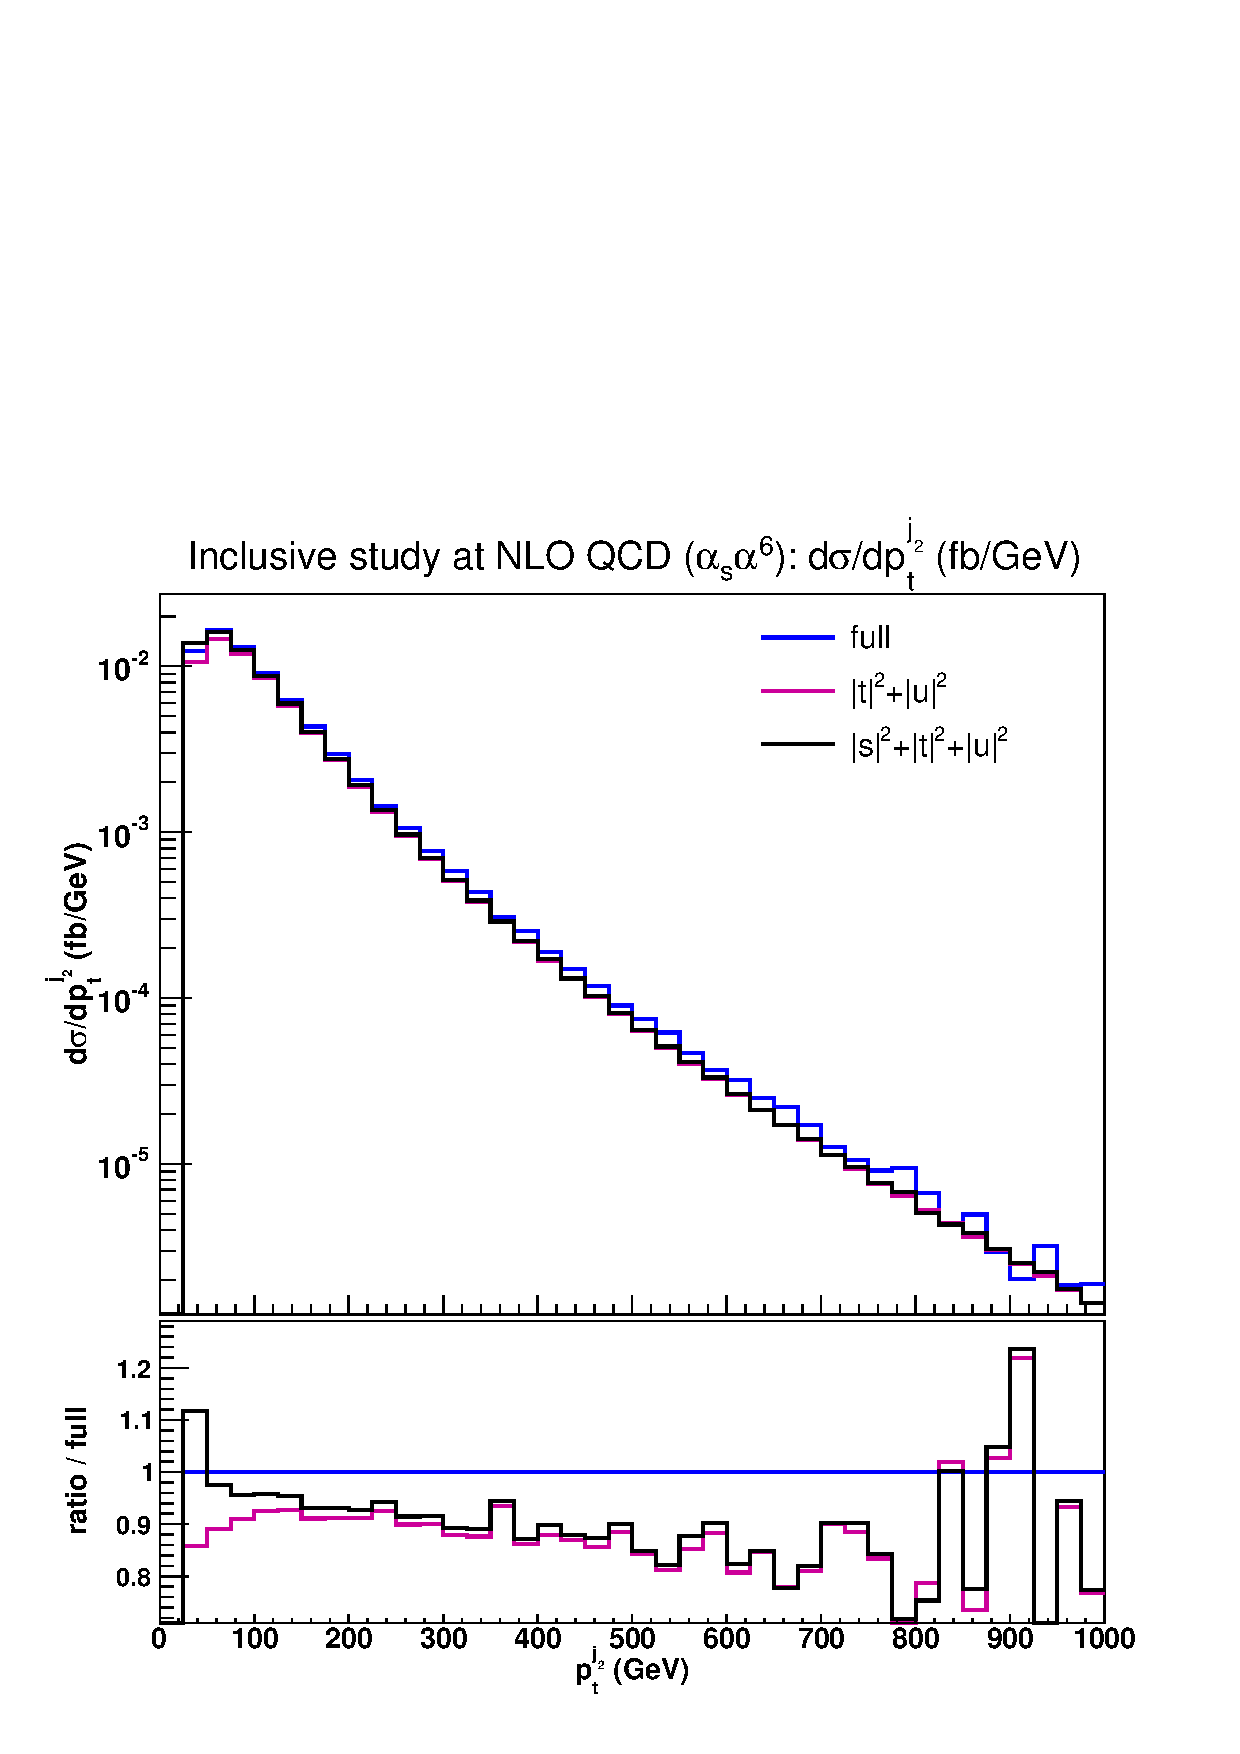
\includegraphics[scale=0.35]{ptj2_nlo.pdf}}
\caption{NLO QCD inclusive study: $p_t$ distributions of the two leading jets, obtained with full ({\sc Recola}) and approximated ({\sc Vbfnlo, Bonsay}) amplitudes at order $\mathcal{O}(\alpha^6\alpha_s)$.} \label{fig:mjjdyjj_1d_2}
\end{figure}

\begin{figure}[hbt]
\centering
\fbox{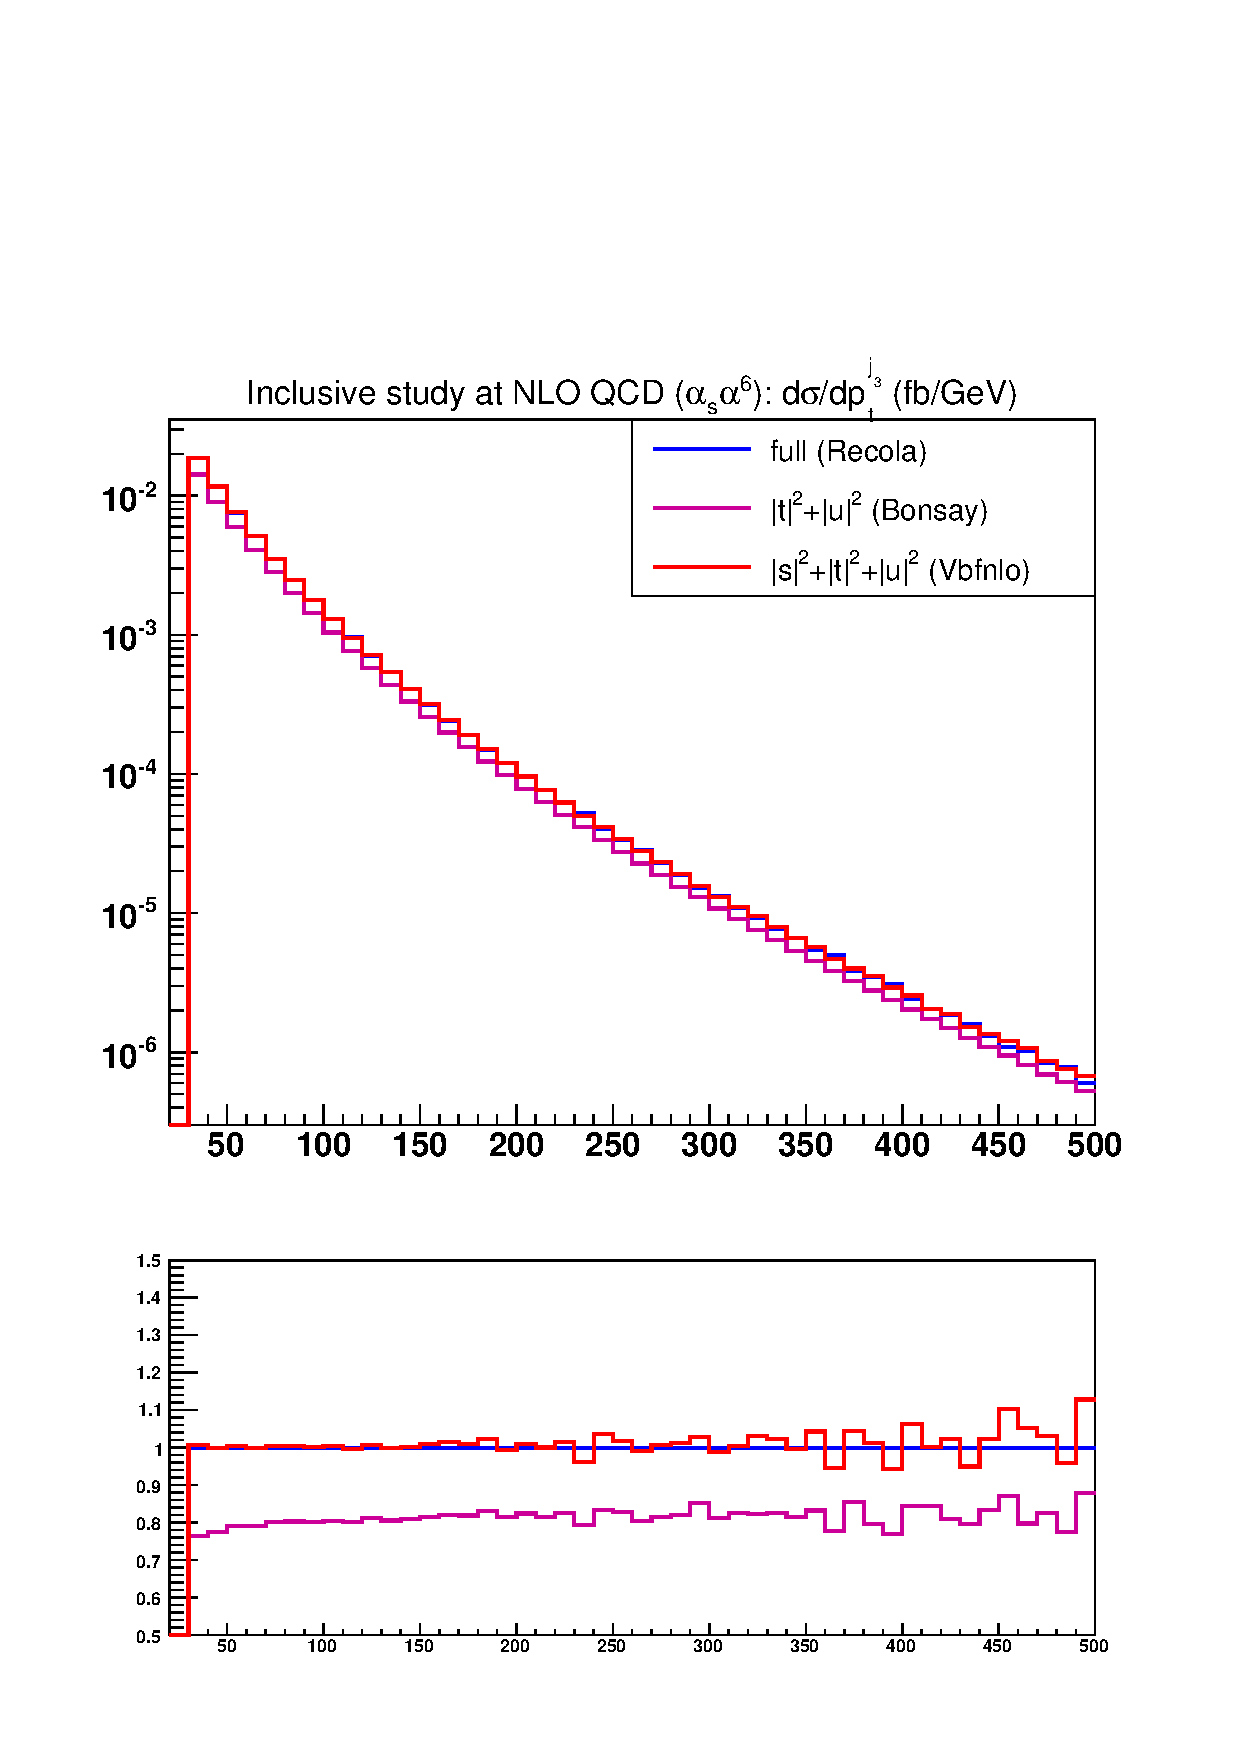
\includegraphics[scale=0.35]{ptj3_nlo.pdf}}
\fbox{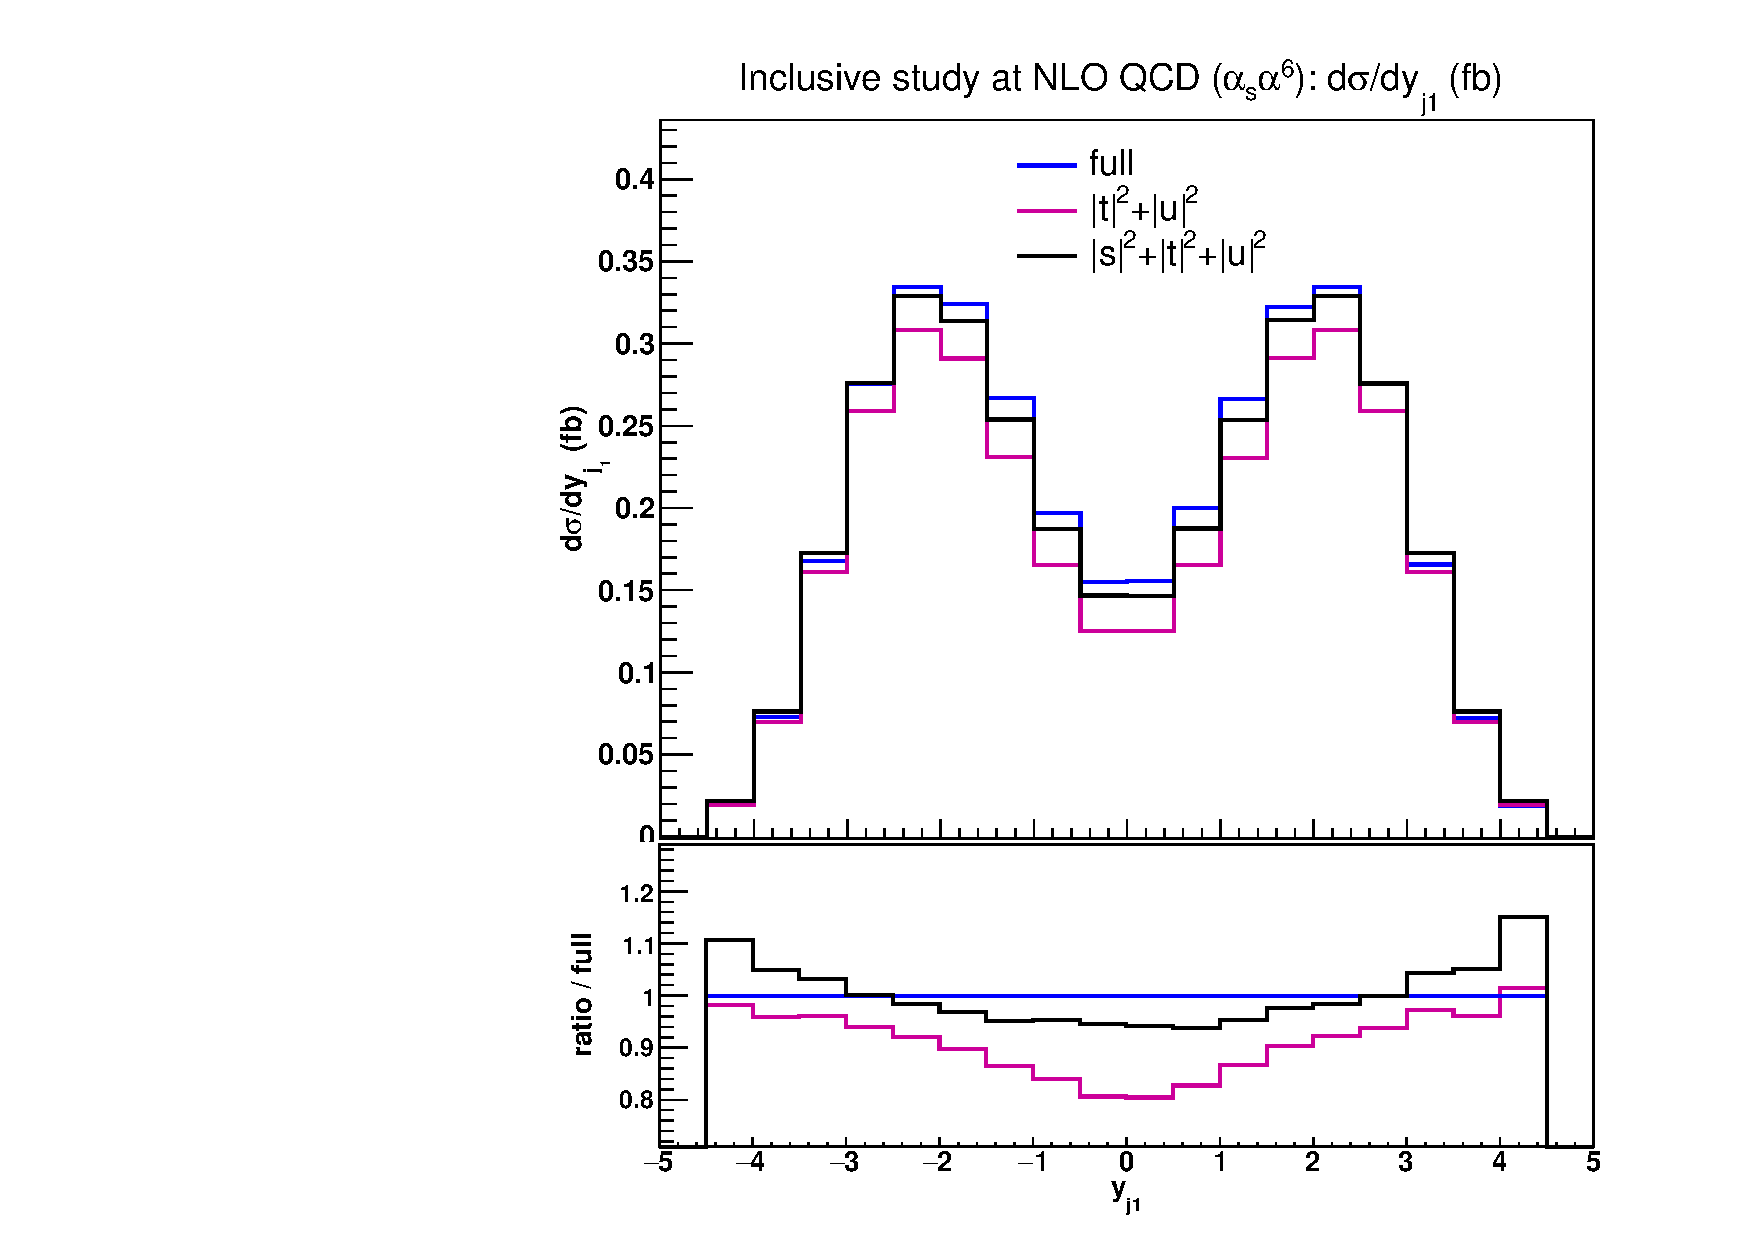
\includegraphics[scale=0.35]{yj1_nlo.pdf}}
\fbox{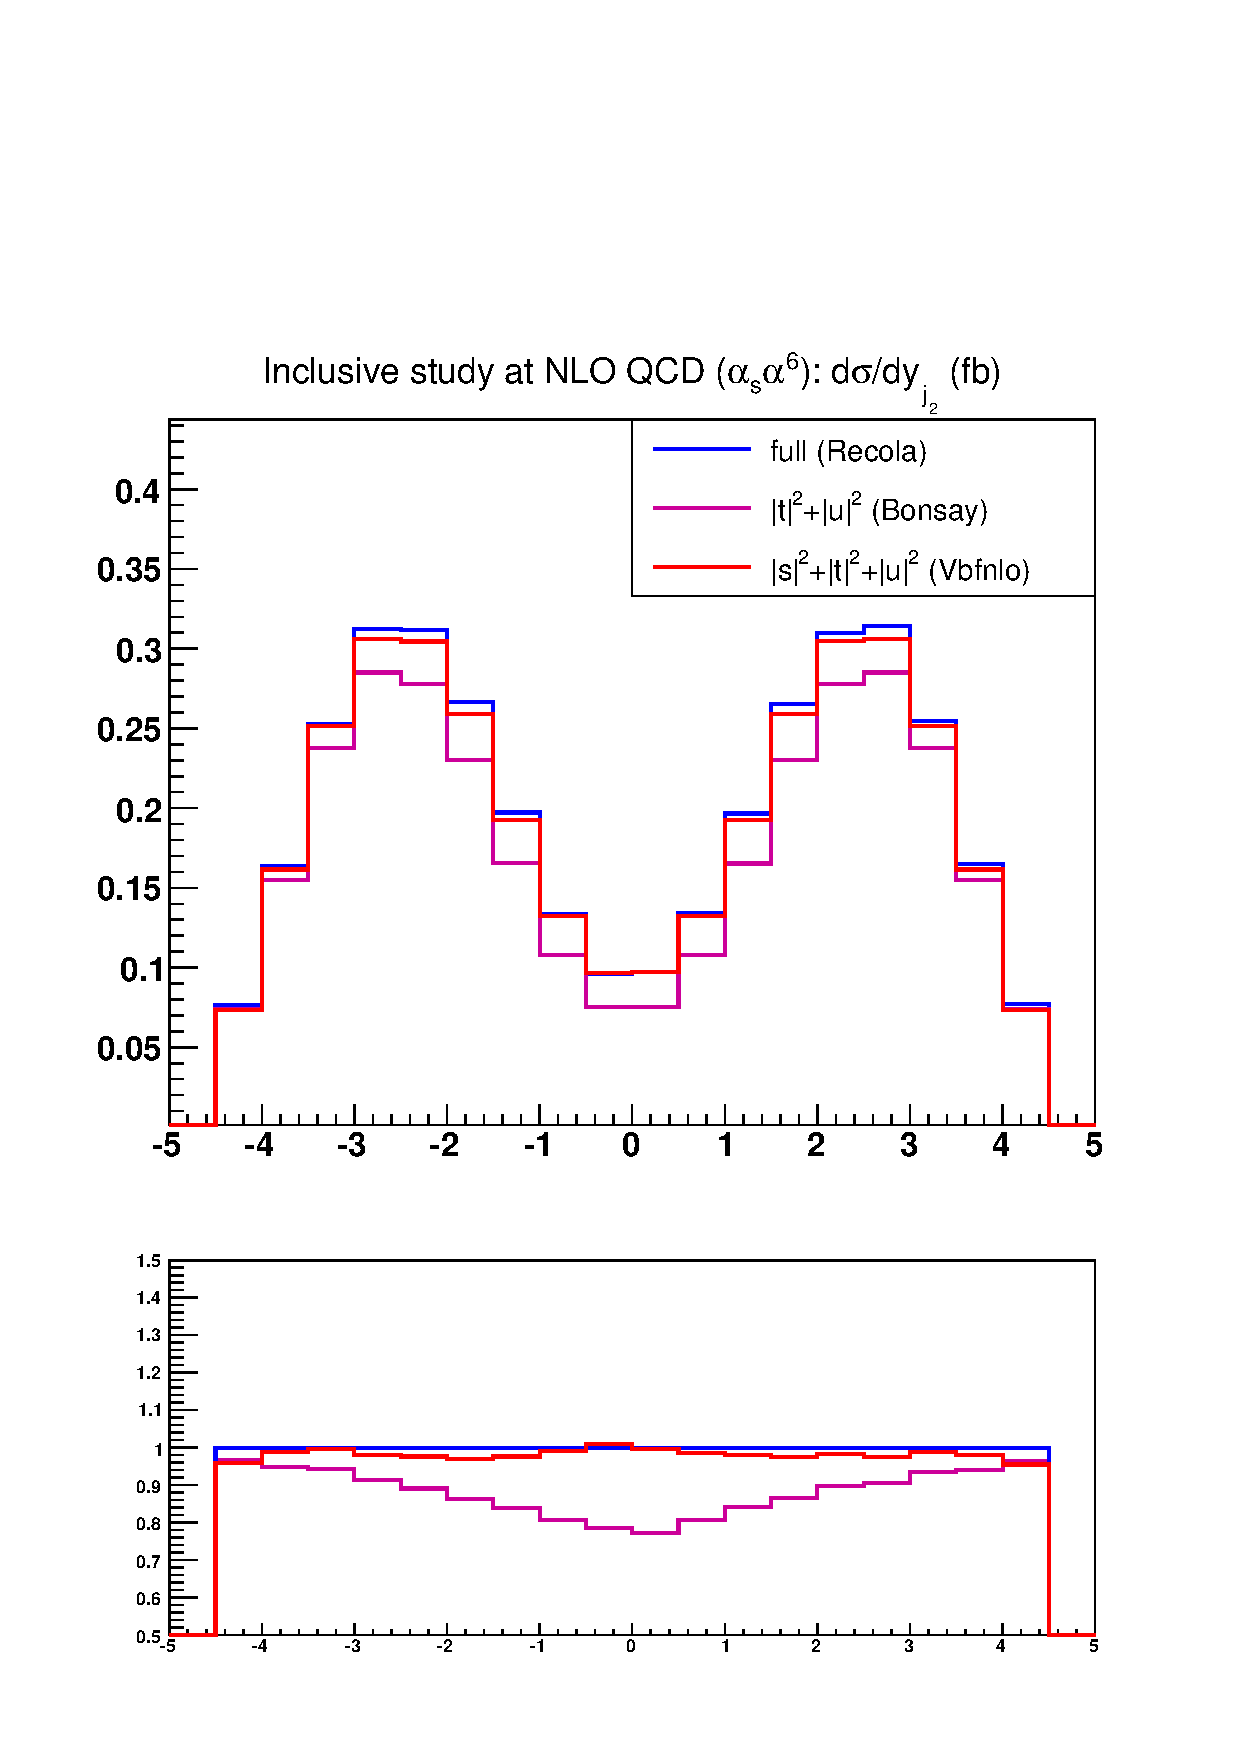
\includegraphics[scale=0.35]{yj2_nlo.pdf}}
\fbox{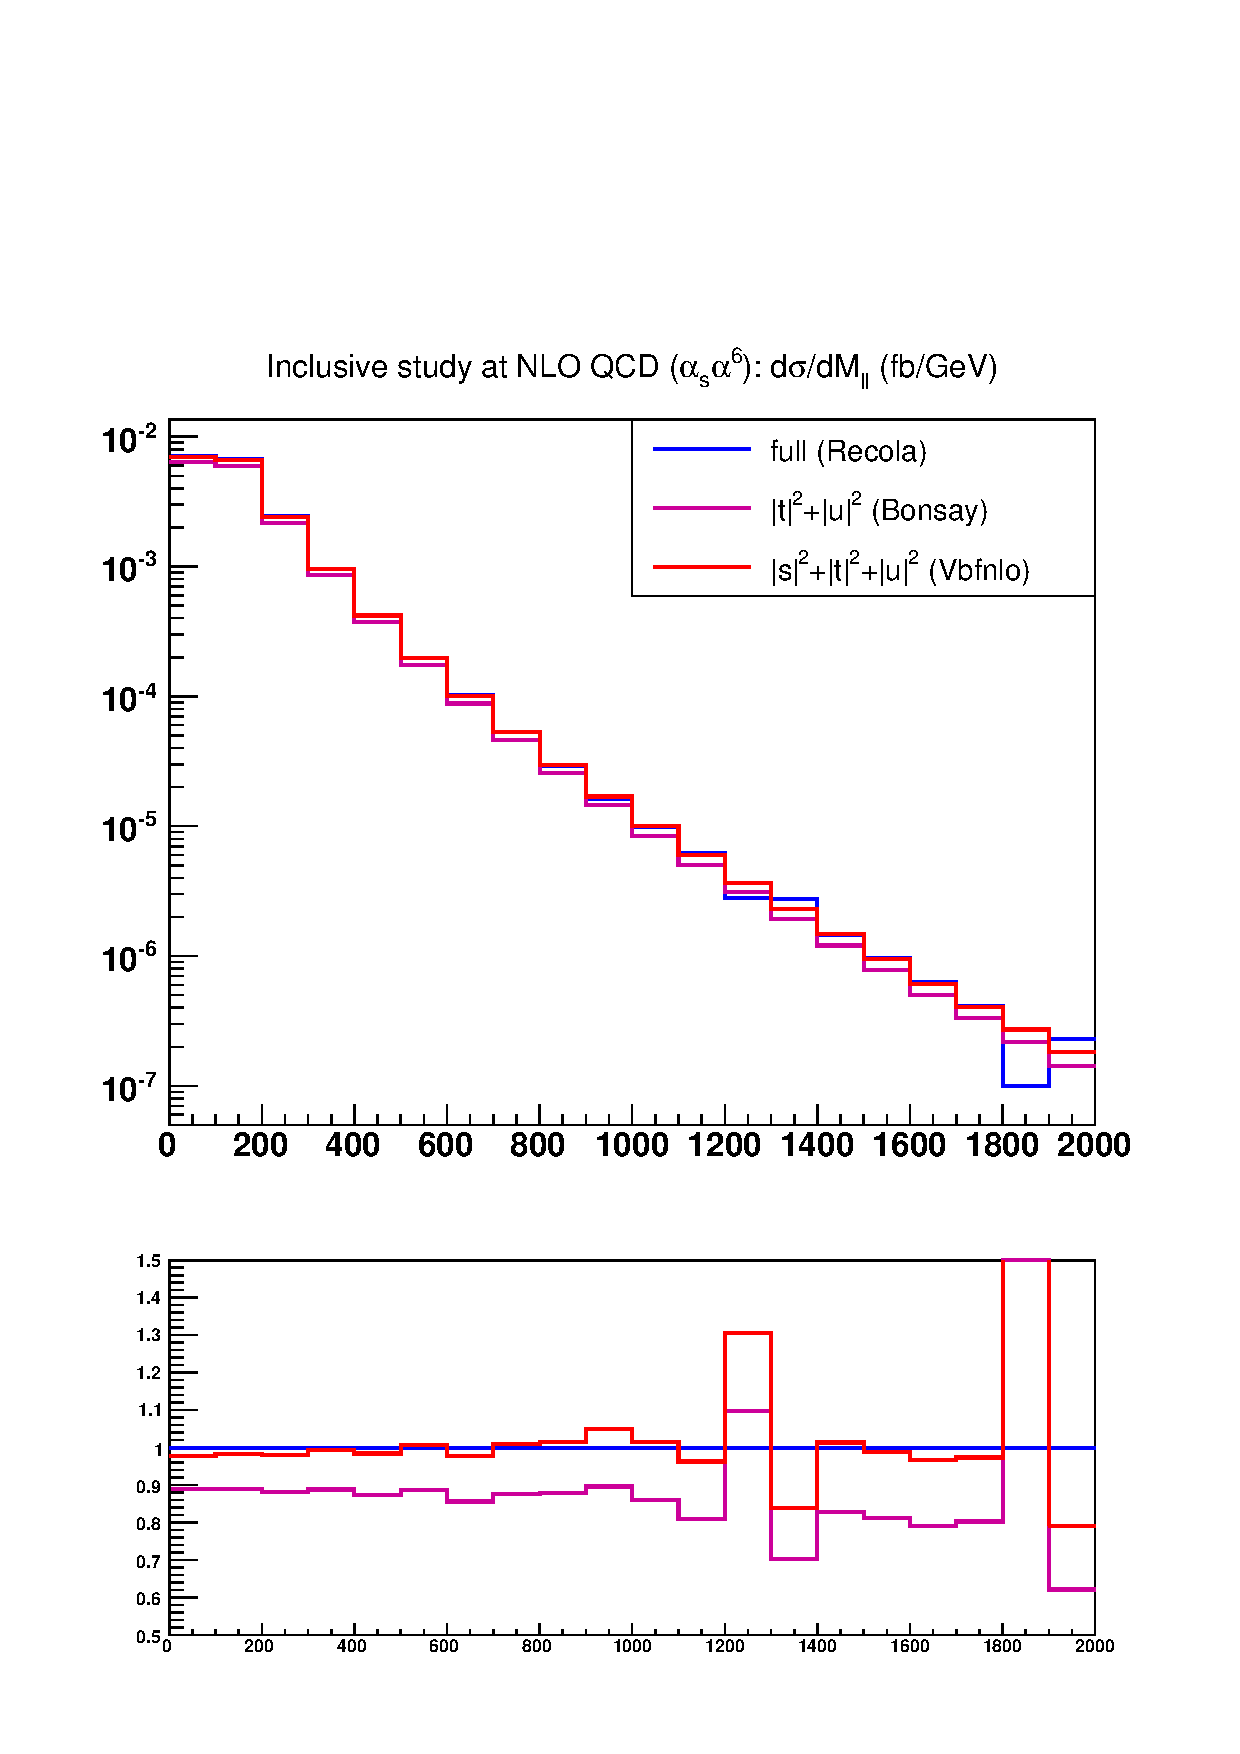
\includegraphics[scale=0.35]{mll_nlo.pdf}}
\fbox{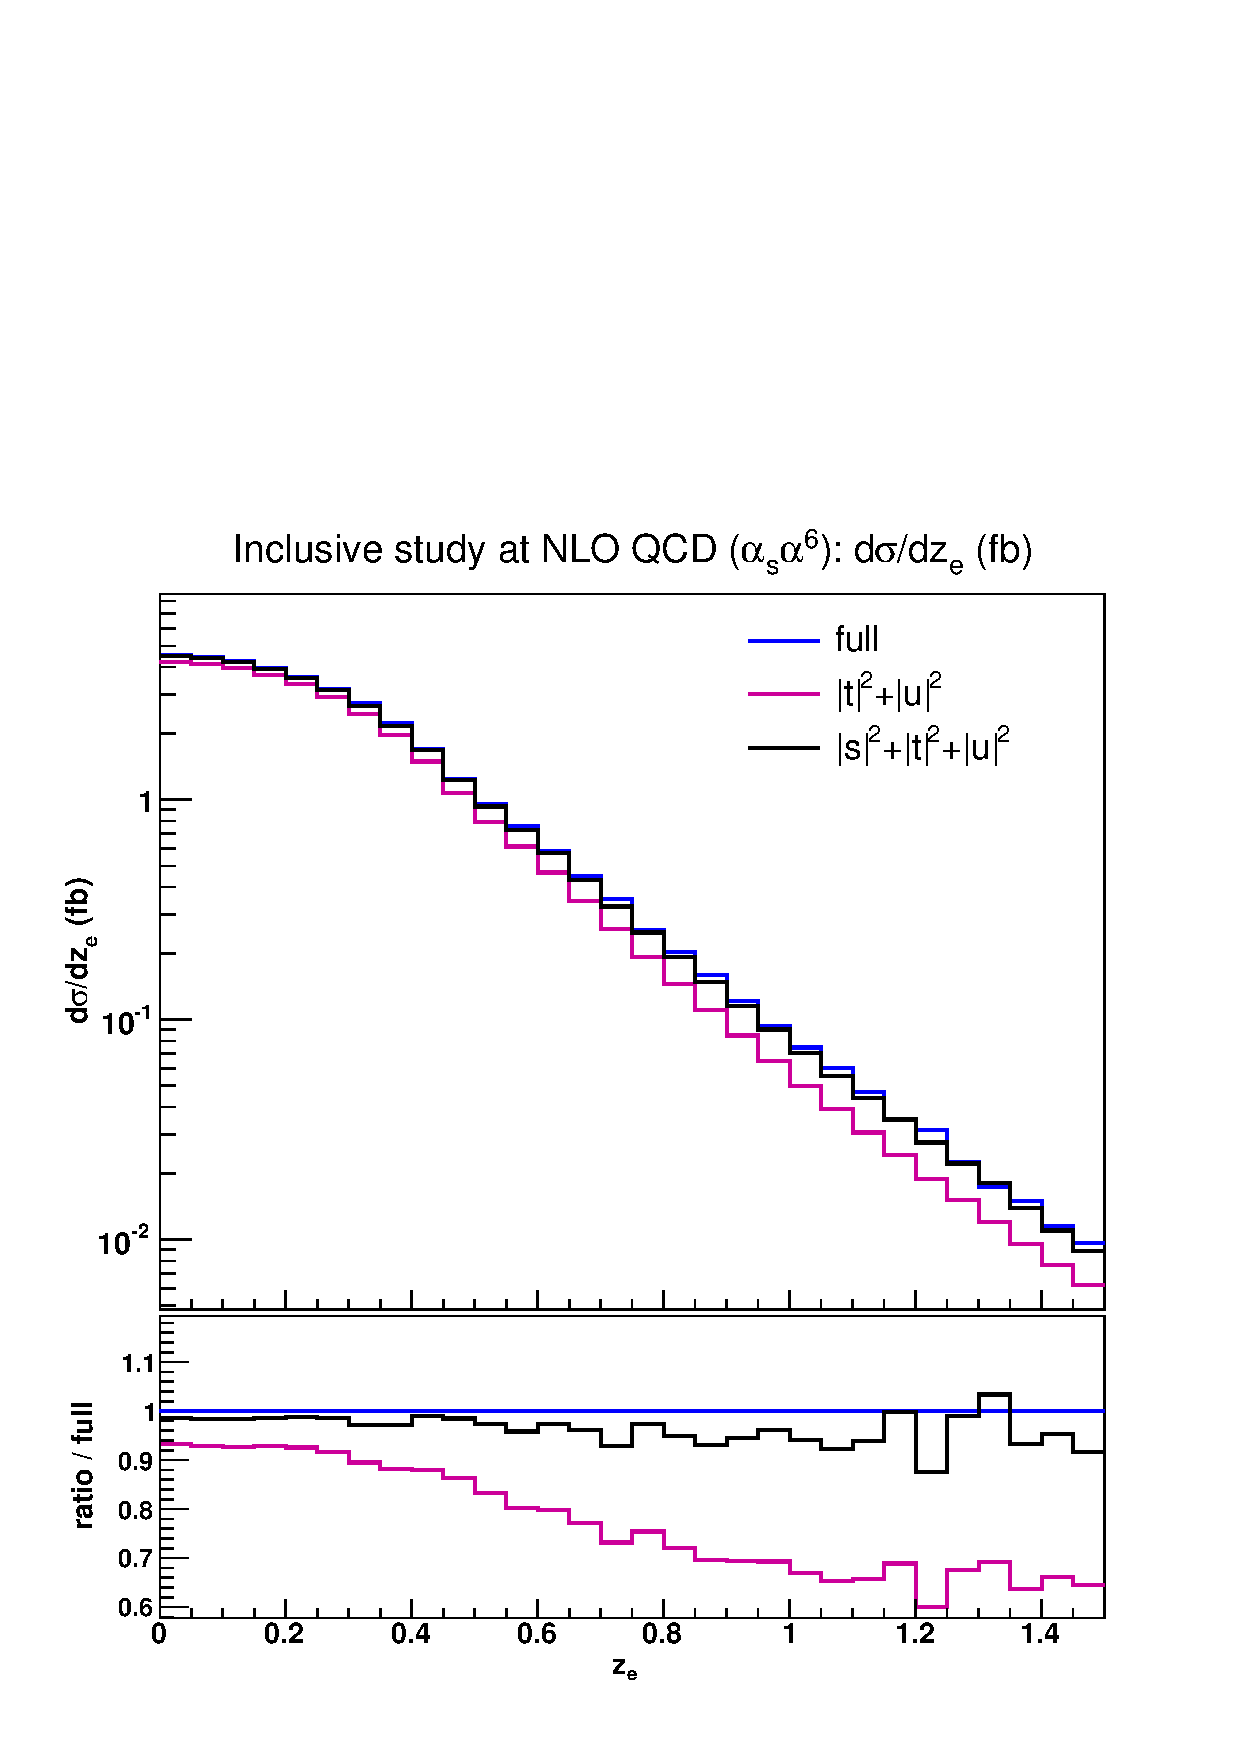
\includegraphics[scale=0.35]{zel_nlo.pdf}}
\fbox{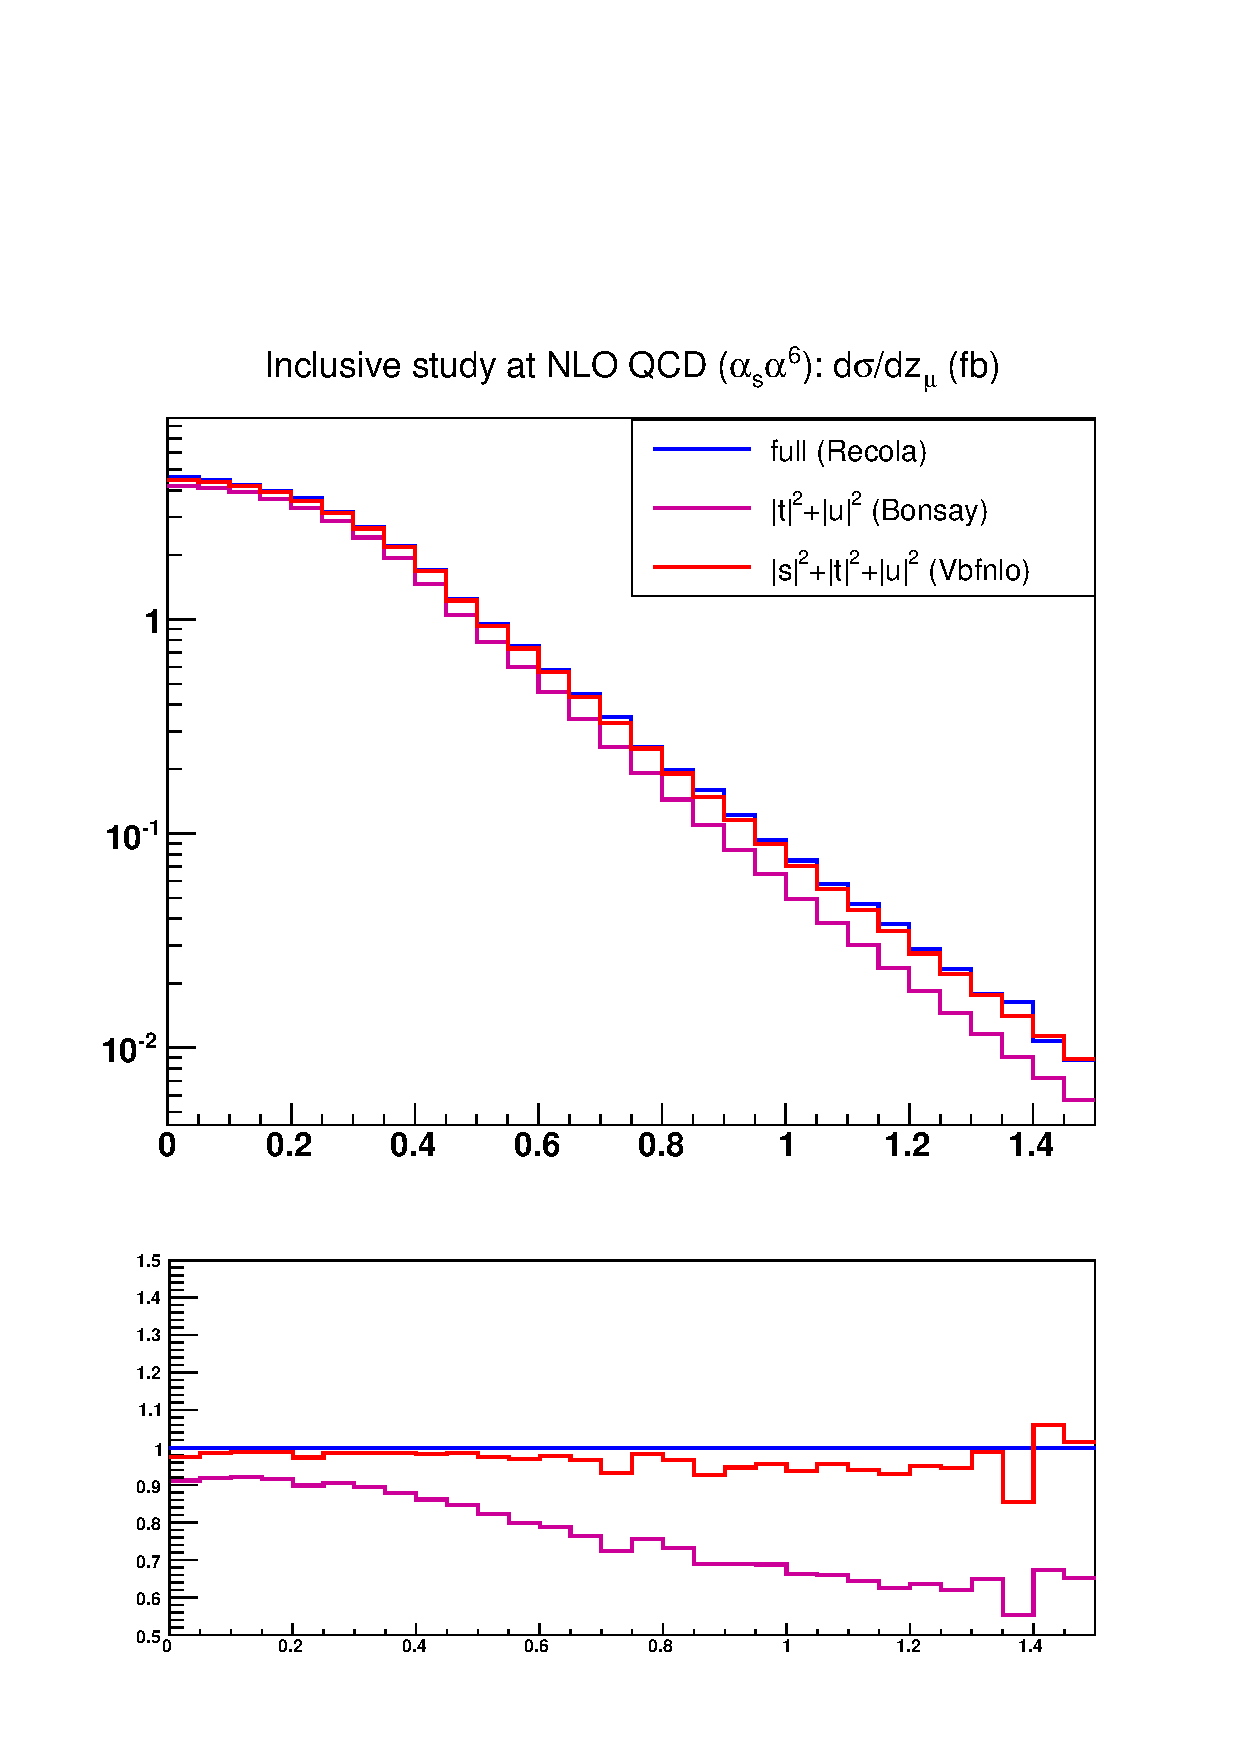
\includegraphics[scale=0.35]{zmu_nlo.pdf}}
\caption{{\bf FIGURES STILL TO BE MODIFIED} } \label{fig:mjjdyjj_1d_3}
\end{figure}

{\bf GP: Maybe a separate subsection for the analysis of the third jet kinematics with LO accuracy ?}
